\chapter{\bf Methodology}\label{chap:metho}
\epigraph{\textit{It is not enough to have a good mind, the main thing is to use it well.}}{Ren\'{e} Descartes, \textit{Discourse on the Method}}

\noindent This chapter describes the relevant information to run the WRF-Chem model and to evaluate the simulation results through recommended statistical benchmarks applied for photochemical models. 
The model configuration, the meteorological initial and boundary conditions (IC/BC), and the emission approaches are also presented.
The description of how the anthropogenic and biogenic emissions files were built is included, considering assumptions and their limitations for future projections.
Additionally, measured air data inside the model domain area and its geographical information is described.
Finally, this section describes statistical benchmarks used for the model performance evaluation for September to October 2018.
Statistical results show us the model performance for current conditions and give us an insight about the model precision to simulate the ozone formation.

Impacts of climate change over surface ozone formation preferentially require analyzing multiyear ensemble simulations.
However, a coupled atmosphere-chemistry model demands high computing time to do this task.
Due to this computational limitation, five years of data (2014-2018) was analyzed to review historical ozone measurements in the S\~{a}o Paulo state. 
After that, as an alternative way, we chose only two months when high surface ozone episodes frequently occurred as a worst-case scenario.
September and October represent these two months in the spring season when higher ozone concentrations are measured due to low cloud cover and high frequency of sunny days, also consistent with findings of \citet{Carvalho2015}.

2018 was chosen as a period that represents current conditions.
Based on the air quality report published by \citet{CETESB2019}, that year presented a high percentage of good air quality conditions than previous years (2014-2017) due to few days of meteorology conditions that enhanced ozone formation.
Only September and December 2018 had a high number of frequent violations of S\~{a}o Paulo air quality standard for ozone (140~$\mu$g~m$^{-3}$, 8-h rolling mean).
June, August, and October did not have exceedances of the air quality standards for ozone.
Nonetheless, the same report mentioned that there isn't a tendency for many years due to photochemical reactions depending on many factors, which have a non-linear relation.

Two scenarios were analyzed using the meteorological datasets as meteorological IC/BC based on the RCP~4.5 (stabilization scenario) and the RCP~8.5 (worst-case scenario) for two month (2030) as future projections.
Only the current simulation for short periods of the year 2018 (Sep. and Oct.) was evaluated through statistic parameters for meteorology and surface ozone concentrations based on recommended statistical benchmarks for photochemical models.
To isolate the effects of changes in future weather conditions, these three sets of simulations (current and future) share the same anthropogenic emission files and geographical data (i.e., land use/land cover, topography height). This means that any variation on future simulations is caused by the weather conditions' effects, affecting the biogenic emissions inside the WRF-Chen due to they depend on the temperature \citep{Guenther2006}.

However, the same chemical boundary conditions, adding the same anthropogenic emissions, and geographical data may cause uncertainty in the model results for future scenarios.
Likewise, according to \citet{VanVuuren2011a}, land use influences the climate system due to interactions with the local atmosphere (i.e., albedo and surface roughness) and biogenic emissions.
For that reason, only the year 2030 was analyzed instead of include the year 2050 or even more future years, considering land use and anthropogenic emission could change in the future, and the uncertainty may increase significantly for 2050.  

\section{Model description and experiment design}
The Weather Research and Forecasting with chemistry model (WRF-Chem) \citep{Grell2005} is an open-source community model, developed by many different groups.
Several research institutes collaborated for the development of the meteorology model Weather Research and Forecasting (WRF) in 1990 through a partnership of the National Center for Atmospheric Research (NCAR), the National Oceanic and Atmospheric Administration (NOAA) -represented by NCEP and ESRL-, the United States Air Force, the Naval Research Laboratory, the University of Oklahoma, and the Federal Aviation Administration \citep{Skamarock2019}.
The WRF model is an Eulerian non-hydrostatic designed for use in atmospheric research and operational forecasting.
Many options of physical parameterizations let us represent subgrid processes that the model cannot explicitly calculate.
Details about WRF meteorological module can be found in \citet{Skamarock2019}.

The model integrates the meteorological and chemical modules. 
The mass coordinate version called Advanced Research WRF (ARW) is the only dynamical core coupled to the chemical module.
To summarize, ARW's equations are cast in flux form from conserved variables; non-conserved variables such as pressure and temperature are diagnosed from the conserved prognostic variables \citep{Grell2005,Skamarock2019}. 
As mentioned by \cite{Skamarock2019}, the main features of the ARW system (version 4) are:

\begin{itemize}
  \item \textit{Equations}: Fully-compressible. Conserves dry air mass and scalar mass.
  \item \textit{Prognostic variables}: Velocity components, and perturbation variables. Optionally, turbulent kinetic energy and any number of scalars.
  \item \textit{Vertical coordinate}: Terrain-following. Top of the model is a constant pressure surface.
  \item \textit{Horizontal grid}: Arakawa C-grid staggering.
  \item \textit{Time integration}
  \item \textit{Spatial discretization}: 2nd- to 6th-order advection options in horizontal and vertical.
  \item \textit{Turbulent mixing and model filters}
  \item \textit{Initial conditions}: Three dimensional for real-data.
  \item \textit{Lateral, top and bottom boundary conditions}
  \item \textit{Earth's rotation}: Full Coriolis terms included.
  \item \textit{Mapping to sphere}: polar stereographic, Lambert conformal, Mercator, and latitude-longitude. Curvature terms included.
  \item \textit{Nesting}: One-way, two-way, and moving nests.
  \item \textit{Nudging}: Grid, spectral, and observation nudging capabilities.
  \item \textit{Global grid}: Global simulation capability.
  \item \textit{Tropical channel}.
\end{itemize}

The physic parameterizations of the model are summarized as follow \cite{Skamarock2019}:

\begin{itemize}
	\item \textit{Microphysics}: They are related to the development of hydrometeors such as water vapor, cloud (ice crystals), and precipitation processes (rain drops) based on how the size distributions of particle types are represented. They are extremely important in climate modeling and their performance can depend on season and the meteorological process that prevail in specific geographic regions \citep{Warner2011}.
	\item \textit{Cumulus parameterizations}: Deep and shallow convection, adjustment, mass-flux, and scale aware schemes available.
	\item \textit{Surface physics}: Multi-layer land surface models ranging from a simple thermal model to full vegetation and soil moisture models, including snow cover and sea ice. Urban parameterizations are available.
	\item \textit{Planetary boundary layer physics}: Turbulent kinetic energy prediction or non-local \textit{K} schemes.
	\item \textit{Atmospheric radiation physics}: Longwave and shortwave schemes with multiple spectral bands and a simple shortwave scheme suitable for climate and weather applications. Cloud effects and surface fluxes are included.
\end{itemize}

The physical and chemical atmosphere processes have interactions that affect meteorological conditions (e.g., clouds and precipitation) and air pollutants concentrations (i.e., ozone, nitrogen oxides, carbon monoxide, aerosols).
For instance, the chemistry can also affect the meteorological conditions through its effect on the radiation budget and aerosols' interaction with cloud condensation nuclei \citep{Grell2005}.

The WRF-Chem model considers those interactions; for that reason is an "online" model. 
The chemistry module is integrated simultaneously with the meteorology module, allowing both components to have the same transport scheme (mass and scalar preserving), the same grid, the same physics options \citep{Grell2005}.
However, this coupled can demand high computational time to resolve physical and chemical processes.
% For that reason, different chemical mechanisms and parameterizations involve resolved-scale variables, replacing processes that cannot be represent directly in a model due to different factors \citep{Warner2011}: small scales, the complexity of a process, and insufficient knowledge about how a process works. % We are not taking about details 
As mentioned by \cite{Grell2005} about the first version of WRF-Chem,
\begin{quote}
    "the chemistry package consists of dry deposition, biogenic emission, the chemical mechanism from RADM2, a complex photolysis scheme, and a state of the art aerosol module (MADE/SORGAN aerosol parameterization)."
\end{quote}
The details of the chemical aspects are covered in \citet{Zaveri1999}, \cite{Grell2005}, \cite{Fast2006}, and \cite{Gustafson2007}.
So, the selection of chemical mechanisms and parameterizations will depend on the study's aims (i.e., secondary aerosol or ozone formation, or both).

\subsection{Model configuration}
The WRF-Chem model (version 4.1.3) simulated three scenarios.
A control period (September and October 2018) was denoted as "current" and two simulations for September and October 2030 for RCP 4.5 and RCP8.5 were named as "future."

Model configurations with two nested domains were used where the MASP is at the center of the domains (Figure~\ref{fig:domain_area}), a 15-km resolution parent, and a 3-km resolution in a one-way concurrent run domain.
This design was chosen because the spatial resolution of meteorology lateral boundary conditions (LBC) for future conditions has one degree, and it is necessary to reduce  errors from the dynamical downscaling procedure.
According to \citet{Warner2011}, there is evidence of errors in regional downscaling modeling due to meteorological LBC.
Thus, the second domain is located far away from the boundary of the parent modeling domain borders.

As mentioned by \citet{Vara2013}, model configurations for 3-km resolution represented better the ozone formation than 1-km resolution.
Therefore, only the 3-km resolution domain was analyzed in this study.
Table~\ref{tab:config} shows the WRF-Chem configuration for these two domains.
The gas-phase chemical mechanism set up in the model is the CBM-Z \citep{Zaveri1999} without Dimethylsulfide (DMS). 
This mechanism was used to simulate tropospheric ozone formation according to findings in \citet{Andrade2015, Gavidia2018} for the MASP conditions. 
This chemical mechanism was chosen due to the use of ethanol as fuel consumption in the MASP.

For running the WRF-Chem model, we started with two days of first spin-up with five days of data analyzed.
We continued the simulation with one day of spin-up, reinitializing meteorology with previously calculated chemistry.
This means that IC is updated every five days of simulation, preserving the previous calculated chemical species concentrations (i.e., chemical IC is not used).
This kind of run helps us to reduce meteorological IC error in our long time simulations.

For instance, as shown in Figure \ref{fig:run}, two days (August 30-31) of spin-up were considered in the WRF-Chem model as a suggestion by \citet{Warner2011}.
The term "spin-up" means generating a model solution of features not entered by the initial conditions such as inertia-gravity waves to reach approximate hydrostatic and geostrophic balance \citep{Warner2011}.
For initialization (red cells), an additional 24 hours before the five days (blue cells) is needed to avoid the adverse effects due to newly meteorology initial conditions.
This last consideration of the temporal modeling setup was based on suggestions by \citet{Ritter2013}, who used 12 hours before the 5-day steps.

\newpage
%\begin{center}
\begin{ThreePartTable}
\begin{TableNotes}
{\scriptsize
	\item[(a)] This configuration uses information from the WRF-Chem Model User's Guide \citep{Wang2019} and WRF-Chem version 3.9.1.1 User's Guide \citep{NOAA2018}.
	\item[(b)] NCEP-FNL (ds083.2) and NCAR CESM (ds316.1) have 32 and 27 metgrid levels, respectively.}
\end{TableNotes}
\footnotesize
\setcaptionmargin{1cm}
\begin{longtable}[c]{l p{0.25\textwidth}l l}
\caption[WRF-Chem model configuration]{WRF-Chem model configuration}\\
\hline
\multicolumn{1}{l}{\bf Description} &
\multicolumn{1}{l}{\bf Option} &
\multicolumn{1}{l}{\bf WRF codes}\\
\hline \endfirsthead
\multicolumn{3}{c}{\footnotesize{{\slshape{{\tablename} \thetable{}}} WRF-Chem model configuration (cont\ldots)
}}\\
\hline
\multicolumn{1}{l}{\bf Description} &
\multicolumn{1}{l}{\bf Option} &
\multicolumn{1}{l}{\bf WRF codes}\\ 
\hline \endhead
\multicolumn{3}{r}{{\scriptsize{Continued on the next page\ldots}}}\\
\endfoot
\hline
\insertTableNotes\\
\endlastfoot
\label{tab:config}
% End of headers and footers
{\bf Domain configuration
\tnote{(a)}
}\\
Points to the west-east direction & 90, 151 & \verb|e_we|\\
Points to the south-north direction & 60, 121 & \verb|e_sn|\\
Vertical levels \tnote{(b)} & 32, 27 & \verb|num_metgrid_levels|\\
Geographical dataset & 30 seg, 30 seg \\
Grid spacing of first domain & 15 km & \verb|dx = 15000, dy = 15000|\\
Grid spacing of second domain & 3 km & \verb|dx = 3000, dy = 3000|\\
Map projection & Mercator & \verb|map_proj = 'mercator'|\\
Center latitude & -23.57 & \verb|ref_lat=-23.57|\\
Center longitude & -46.61 & \verb|ref_lon=-46.61|\\
{\bf Physical parameterizations}\\
Long-wave radiation & RRTM & \verb|ra_lw_physics=1, 1|\\
Short-wave radiation & RRMG & \verb|ra_sw_physics=4, 4|\\
Boundary layer & BouLac & \verb|bl_pbl_physics=8, 8|\\
Surface layer & Revised MM5 scheme & \verb|sf_sfclay_physics = 1, 1|\\
Land-surface & Noah & \verb|sf_surface_physics=2, 2|\\
Cumulus cloud & Grell 3D & \verb|cu_physics=5, 5|\\
Cloud microphysics & Morrison~double-moment scheme & \verb|mp_physics=10, 10|\\
Urban surface & Urban canopy model & \verb|sf_urban_physics=1|\\
{\bf Chemical options}\\
Chemical lateral & Idealized profile  & \verb|chem_in_opt=0|\\
 & re-initialization & \verb|chem_in_opt=1|\\
Gas-phase mechanism & CBMZ without DMS & \verb|chem_opt=6, 6|\\
Photolysis scheme & Fast-J & \verb|phot_opt=2|\\
Emissions & Two 12 h files & \verb|io_style_emissions=1|\\
 & CBMZ/MOSAIC anthropogenic emissions & \verb|emiss_opt=4, 4|\\
 & RADM2 speciation & \verb|emiss_inpt_opt=102, 102|\\
 & MEGAN2 & \verb|bio_emiss_opt=3|\\
 &  & \verb|ne_area = 70|\\
 & No GOCART dust emissions & \verb|dust_opt=0|\\
 \hline
\end{longtable}
\end{ThreePartTable}
%\end{center}
	
\begin{figure}[htbp]
  \includegraphics[width=1\textwidth]{fig/Domain.pdf} %\llap{\raisebox{9.2cm}{\includegraphics[width=0.2\textwidth]{fig/world_area.pdf}}}
  \caption{WRF-Chem simulation domain}
  {\scriptsize Notes: \\ The MASP is at the center of the domain area (23.5ºS and 46.6ºW) in the São Paulo state. The height ground terrain was based on \verb|geo_em.d01.nc| and \verb|geo_em.d02.nc|, generated both by WPS Preprocessor.}
  \label{fig:domain_area}
\end{figure}

\begin{figure}[htbp]
  \includegraphics[width=1\textwidth]{fig/WRFrun.pdf} %\llap{\raisebox{9.2cm}{\includegraphics[width=0.2\textwidth]{fig/world_area.pdf}}}
  \caption{WRF-Chem simulation for September and 2030}
  {\scriptsize Note: \\ Green cells are two days of spin-up; blue cells are data output analyzed for this study; red cells are one day of spin-up for meteorology initialization.}
  \label{fig:run}
\end{figure}

	\begin{figure}[htbp]
		\begin{center}
			\includegraphics[width=1\textwidth]{fig/data_flow.pdf}
		\end{center}
		\caption{Flowchart for running the WRF-Chem model, applied to this study}
  		{\scriptsize Note: \\ Geogrid defines the model domain and creates static files of terrestrial data. Ungrib: decodes GRIB-formatted data only for global data for 2018. Metgrid: interpolates meteorological data to the model domain. Emission files are generated from LAPAt preprocessor emissions through the Bottom-up method for road transport (Sep. and Oct. 2018), adding industry and residential emissions from EDGAR-HTAP (2010) using ANTHRO\_EMISS.  LBC: Lateral-Boundary Conditions; IC: Initial Conditions. WRF is ran based on Real Data ARW System.}
  		\label{fig:flow}
	\end{figure}
	
The "{\it namelist.wps}" controls the WRF Preprocessor System (WPS) configuration while the "{\it namelist.input}" controls WRF configuration (Figure \ref{fig:flow}).
Both namelists are shown in Appendix \ref{ap03}.
The WPS module prepares geography and meteorology data based on the modeling domain area.
Geography data has limitations because it can not represent current features for years 2018 and 2030.
However, the WPS used the high resolution available (30s) from MODIS and USGS data, downloaded from the \href{https://www2.mmm.ucar.edu/wrf/users/download/get_sources_wps_geog.html}{WRF webpage}.
In the WRF module, the namelist.input requires chemical options that are located in \verb|&chem| section, like the chemical mechanism, the biogenic emission scheme, or the chemical LBC. 
Different from a meteorological run, WRF-Chem requires emission files in NetCDF format, called `wrfchemi'.
The real.exe builds initial ({\it wrfinput\_<domain>}) and lateral-boundary conditions ({\it wrfbdy\_d01}).
Finally, wrf.exe uses IC/BC and the emission files to simulate hourly meteorological variables and pollutant concentrations in the defined spatial resolution.
 After running the first seven days (Figure~\ref{fig:run}), re-initialization uses {\it wrf\_chem\_input\_d01} and {\it wrf\_chem\_input\_d02} linked to the first hour of the previous day, using Linux codes, for instance:
  \\ \verb|ln -sf ../wrfout_reinit/wrfout_d01_2018-09-05_00:00:00 wrf_chem_input_d01|\\
  \verb|ln -sf ../wrfout_reinit/wrfout_d02_2018-09-05_00:00:00 wrf_chem_input_d02|\\
 Also, it is necessary edit options in the namelist.input:
 \begin{verbatim}
 	io_form_auxinput12 = 2
 	auxinput12_inname = `wrf_chem_input'
 	chem_in_opt = 1, 1
 \end{verbatim}
	
	
	\subsection{Initial and Lateral-Boundary Conditions (IC/BC)}
	
		\subsubsection{Meteorology IC/BC}
		For the `current' scenario (Sep-Oct 2018), the WRF-Chem model was initialized from the NCEP Final Analysis (available online at \href{https://rda.ucar.edu/datasets/ds083.2/}{ds083.2}), which has a temporal resolution of six hours and a horizontal resolution of 1 $\times$ 1 degree.
		According to \cite{NCEP2000}, parameters include surface pressure, sea level pressure, geopotential height, temperature, sea surface temperature, soil values, ice cover, relative humidity, zonal (u) and meridional (v) winds, vertical motion, vorticity and ozone.
		
		For the `future' scenario (Sep-Oct 2030), the model was initialized from the NCAR's Community Earth System Model (CESM1) outputs with 1 $\times$ 1 degree resolution every six hours (available online at \href{https://rda.ucar.edu/datasets/ds316.1/}{ds316.1}).
		CESM1 participated in phase 5 of the Coupled Model Intercomparison Experiment (CMIP5) \citep{Monaghan2014}, which supported the Intergovernmental Panel on Climate Change (IPCC) Fifth Assessment Report (AR-5).
		Two datasets for future scenarios based on RCP~4.5 and RCP~8.5 were used.
		These contain all the variables needed for the meteorological IC/BC for simulations with WRF-Chem, provided in the Intermediate File Format specific to WRF. This means that running "{\it ungrib}"\footnote{Extract meteorological fields from {\it GRIB} files.} in WPS is not required.
		The variables have been bias-corrected using the European Centre for Medium-Range Weather Forecast (ECMWF) Interim Reanalysis (ERA-Interim).
		The datasets have 26 pressure levels and the meteorological variables are air temperature, boundary-layer winds, geopotential height, humidity, sea ice concentration, sea level pressure, sea surface temperature, skin temperature, snow water equivalent, soil moisture/water content, soil temperature, surface pressure, surface winds, upper-air temperature, upper-level winds.
		
		\subsubsection{Chemical IC/BC}
		According to \citet{Gavidia2018}, dynamic chemical BC affects more ozone simulation with WRF-Chem in the autumn season (May) than in the spring season when photochemical activity is a higher. 
		The same authors show in their results that the impact of dynamic chemical conditions could be neglected when the photochemical activity is higher (e.g., spring season).
		The study concludes that the dynamic chemical BC does not significantly impact near-surface ozone concentration due to ozone formation much depending on the vehicular emission.
		For that reason, this study considered chemical BC based on the default configuration.
		
		According to \citet{Grell2005} and WRF-Chem User's Guide, default chemical IC/BC are based on northern hemispheric, mid-latitude, clean environment conditions with data based upon results from a NOAA-Aeronomy Laboratory Regional Oxidation Model (NALROM).
		For the initial simulation period with two days of spin-up, the model was initialized with \verb|chem_in_opt = 0| in the `namelist.input'.
		After that, the re-initialization only applied to meteorological IC/BC and considered the first hour of the previous day based on the WRF-Chem output, preserving the previous calculated chemical species concentrations, as shown in Figure~\ref{fig:run}.
		This procedure was used for `current' and `future' simulations.

	\section{Anthropogenic and biogenic emissions}
	Anthropogenic emissions used as input in the model represent three main sectors (i) road transport, (ii) industry, and (iii) residential.
	For the representation of the transport sector emission it was used the LAPAt pre-processor emissions model \citep{Andrade2015} based on a bottom-up approach for emissions inventory.
	The bottom-up approach provides detailed emission rates with spatial and temporal variation, using local detailed emission factors and activity data \citep{Wang2009}.
	
	For the industry and residential sectors, \verb|anthro_emiss| tool \citep{Kumar2020} was used to assimilate EDGAR-HTAP emissions to our two modeling domains.
	Biogenic emissions were calculated online using the Model of Emissions of Gases and Aerosols from Nature (MEGAN), through \verb|bio_emiss| tool.
	Both tools (\verb|anthro_emiss| and \verb|bio_emiss|) are available on the \href{https://www.acom.ucar.edu/wrf-chem/download.shtml}{NCAR UCAR web page}.
	Appendix~\ref{ap02} presents details about the data source used to generate emission files required by the WRF-Chem model.
	
		\subsection{Road transport emissions}
		
		LAPAt pre-processor emissions model, cited in \citet{Andrade2015}, created the WRF-Chem emission files for road transport based on a bottom-up approach. {\footnotesize
\begin{longtable}{lllr}
\caption{Vehicular fleet by type and fuel for São Paulo State \citep{CETESB2019a}}\label{tab:flota}\\
\toprule
	\textbf{ID} &    \textbf{ Category} & \textbf{Fuel} & \textbf{Veh/year} \\
\midrule
\endhead
\midrule
\multicolumn{4}{r}{{Continued on next page}} \\
\midrule
\endfoot

\bottomrule
\endlastfoot
  VEIC 1 &               Passenger Car (PC) &    Gasoline C &   2686720 \\
  VEIC 2 &               Passenger Car (PC) &       Ethanol &    203893 \\
  VEIC 3 &               Passenger Car (PC) &     Flex-fuel &   7402653 \\
  VEIC 1 &  Light Commercial Vehicles (LCV) &    Gasoline C &    503522 \\
  VEIC 2 &  Light Commercial Vehicles (LCV) &  Ethanol Hid. &     19460 \\
  VEIC 3 &  Light Commercial Vehicles (LCV) &     Flex-fuel &    959325 \\
 VEIC 4A &  Light Commercial Vehicles (LCV) &        Diesel &    427788 \\
 VEIC 4A &                 Light Truck (LT) &        Diesel &     32662 \\
 VEIC 4A &           Semi Light Truck (SLT) &        Diesel &    107579 \\
 VEIC 4A &                Medium Truck (MT) &        Diesel &     61148 \\
 VEIC 4A &           Semi Heavy Truck (SHT) &        Diesel &    112008 \\
 VEIC 4A &                 Heavy Truck (HT) &        Diesel &    124368 \\
 VEIC 4B &            Small Urban Bus (SUB) &        Diesel &     62351 \\
 VEIC 4B &                   Urban Bus (UB) &        Diesel &     15069 \\
 VEIC 4C &      Urban Bus Articulated (UBA) &        Diesel &     28243 \\
 VEIC 6A &                  Motorcycle (MC) &    Gasoline C &   1823493 \\
 VEIC 6B &                  Motorcycle (MC) &     Flex-fuel &    696079 \\
\end{longtable}}
		After running test simulations using different emission rates, we corrected only the emission rates for the road transport sector through a correction factor to achieve simulations closer to performance benchmarks suggested by \citet{Emery2017}.	
		Road transport emission approximation through the LAPAt pre-processor model required the following information:
		
		\begin{itemize}
			\item \textbf{\textit{Road length}}: Two files for each modeling domain (\verb|grid3km_d02.txt| and \verb|grid15km_d01.txt|) represent the sum of motorway, trunk, primary, secondary, and tertiary types of roads inside each grid cell.
			\item \textbf{\textit{Fraction fleet by type and vehicle number}}: Table~\ref{tab:flota} shows fraction fleet by type was obtained from the emission report published by \citet{CETESB2019a}. It is mainly based of fuel type and light or heavy duty vehicles. The vehicle number for September and October 2018 was obtained from  \href{https://www.gov.br/infraestrutura/pt-br/assuntos/transito/conteudo-denatran/frota-de-veiculos-2018}{DENATRAN webpage}. There is a specific information about monthly vehicle numbers by type, for each municipality and state. Two estimations of total vehicle fleet were obtained for the first (56~410~975 vehicles in Sep. 2018 and 56~604~008 vehicles in Oct. 2018) and second (24~259~504 vehicles in Sep. 2018 and 24~332~719 vehicles in Oct.) domain. 
			\item \textbf{\textit{Emission factors}} by vehicle and fuel types were used as shown in Table~\ref{tab:ef} in units of g km$^{-1}$. Different vehicle types (motorcycles, light-duty vehicles, and heavy-duty vehicles) and fuel types (gasohol, ethanol, ethanol-blended gasohol, and diesel) release different pollutant emission rates (CO, NO$_x$, particles, SO$_x$, VOC). 
\begin{table} %[width=.9\textwidth,cols=3,pos=ht]
\begin{threeparttable}[b]
\caption{Emissions factors (g/km) based on \citet{Perez2014} and \citet{Andrade2015, Andrade_agu2019}}\label{tab:ef}
\begin{tabular}{@{} lrrrrrrrrrr @{} }
\toprule
Pollutants \tnote{a} & \multicolumn{3}{l}{Light-duty vehicles \tnote{b}} & \multicolumn{3}{l}{Heavy-duty vehicles \tnote{c} } & Taxis \tnote{d} & \multicolumn{2}{l}{Motorcycles \tnote{e} }  \\ 
\cline{2-10}
            & VEIC 1 & VEIC 2 & VEIC 3                  & VEIC 4A & VEIC 4B & VEIC 4C               & VEIC 5                                   & VEIC 6A & VEIC 6B                 \\ 
\midrule
exa CO     & 4.4000 & 12.000 & 4.4000                  & 1.5000  & 1.5000  & 1.5000                & 0.0000                                   & 9.1500  & 9.0200                  \\
exa CO$_2$    & 219.00 & 219.00 & 219.00                  & 1422.0  & 1422.0  & 1422.0                & 0.0000                                   & 0.0000  & 0.0000                  \\
exa NO$_x$    & 0.2000 & 1.1200 & 0.2000                  & 6.9000  & 6.9000  & 6.9000                & 0.0000                                   & 0.1320  & 0.1290                  \\
exa SO$_2$    & 0.0290 & 0.0140 & 0.0210                  & 0.6100  & 0.6100  & 0.6100                & 0.0000                                   & 0.0097  & 0.0093                  \\
exa C$_2$H$_5$OH & 0.5080 & 0.2500 & 0.5080                  & 0.6100  & 0.6100  & 0.6100                & 0.0000                                   & 0.0790  & 0.3050                  \\
exa HCHO   & 0.0089 & 0.0110 & 0.0098                  & 0.6100  & 0.6100  & 0.6100                & 0.0000                                   & 0.0152  & 0.0155                  \\
exa Aldehyde    & 0.0140 & 0.0300 & 0.0220                  & 0.6100  & 0.6100  & 0.6100                & 0.0000                                   & 0.0164  & 0.0188                  \\
exa PM     & 0.0200 & 0.0200 & 0.0200                  & 0.2770  & 0.2770  & 0.2770                & 0.0000                                   & 0.0500  & 0.0500                  \\
exa VOC    & 0.4250 & 1.3000 & 0.4340                  & 2.0500  & 2.0500  & 2.0500                & 0.0000                                   & 1.0800  & 1.0800                  \\
vap VOC    & 0.2300 & 0.2500 & 0.2400                  & 0.0000  & 0.0000  & 0.0000                & 0.0000                                   & 0.0000  & 0.0000                  \\
liq VOC    & 2.0000 & 1.5000 & 1.7500                  & 0.0000  & 0.0000  & 0.0000                & 0.0000                                   & 1.2000  & 1.2000                  \\
\bottomrule
\end{tabular}
\begin{tablenotes}
{\scriptsize
	\item[a] Exhaust (exa), evaporative (eva), and liquid (liq).
	\item[b] VEIC 1 (gasoline), VEIC 2 (ethanol), VEIC 3 (flex-fuel).
	\item[c] Diesel as fuel: VEIC 4A (semi light, medium, and semi heavy trucks), VEIC 4B (small and urban bus), VEIC 4C (urban bus articulated).
	\item[d] Taxis use natural gas as fuel.
	\item[e] VEIC 6A (motorcycle, gasoline), VEIC 6B (motorcycle, flex-fuel).}
\end{tablenotes}
\end{threeparttable}
\end{table}


			\item \textbf{\textit{Use intensity mean}}: Kilometer traveled by vehicle type (km day$^{-1}$), shown in Table~\ref{tab:use_int}, was calculated based on CETESB information. \begin{table}
\centering
\footnotesize 
\caption{Intensity of use by vehicle type and fuel}
\label{tab:use_int}
\begin{tabular}{lll} 
\toprule
\textbf{Vehicle type}          & \textbf{Fuel}                                                       & \textbf{Use (km/day)}  \\ 
\hline
Light-duty vehicles (VEIC 123) & \begin{tabular}[c]{@{}l@{}}Gasohol\\Ethanol\\Flex-fuel\end{tabular} & 39.39                  \\
Truck (VEIC 4A)                & Diesel                                                              & 91.02                  \\
City buses (VEIC 4B)           & Diesel                                                              & 86.70                  \\
Intercity busses (VEIC 4C)     & Diesel                                                              & 106.18                 \\
Taxis (VEIC 5)                 & Natural gas                                                         & 0                      \\
Motorcycle (VEIC 6A)           & Gasohol                                                             & 32.16                  \\
Motorcycle (VEIC 6B)           & Flex-fuel                                                           & 35.78                  \\
\bottomrule
\multicolumn{3}{l}{\scriptsize Based on available data provided in emission report of \cite{CETESB2019a}.} 
\end{tabular}
\end{table}
			\item \textbf{\textit{Emission correction factor}}: To obtain the best simulation for the current scenario (September 2018), 11 experiments were developed running 5 days with no precipitation (September 6 - 12 and 24 - 28, 2018). The experiment 10 was chosen because they reached two of three (correlation coefficient and normalized mean bias) statistical benchmarks suggested by \citet{Emery2017} for surface ozone. The experiment 10 only required a correction factor for road transport emission (\verb|fc_nox = 0.8|) indicated in the LAPAt pre-processor model.
			\item \textbf{\textit{Temporal distribution}}: Normalized average vehicles counts by light-duty (LDV) and heavy-duty (HDV) were done from the tunnel experiments as is mentioned in \citet{Andrade2015}, shown in Figure~\ref{fig:temp_distr}. 	
	\begin{figure}
		\centering
		\includegraphics[width = .5\textwidth]{fig/Temp_distr.pdf}
  		\caption{Temporal distribution of emissions for light-duty (LDV, including motorcycles) and heavy-duty (HDV) vehicles, according to \citet{Andrade2015}.}
  		\label{fig:temp_distr}
	\end{figure}
			\item \textbf{\textit{Relative fractions of VOC emissions}}: This information was shown in \citet{Andrade2015} related to VOC fractions for exhaust, evaporative, and liquid emissions from gasohol, ethanol, and diesel. The VOC speciation was made considering measurements performed in tunnels and with dynamometers \citep{Perez2014, Nogueira2014}.
		\end{itemize}		
	
	\subsection{Industry and residential emissions}
	Global EDGAR-HTAP \citep{Janssens2015, Crippa2020} emission inventory has data for the year 2010 and by sector (i.e., industry and residential).
	This dataset provides monthly grid maps with a spatial resolution of 0.1$^{\circ}$ x 0.1$^{\circ}$ (latitude by longitude).
	The utility $anthro\_emiss$, Fortran based preprocessor, creates WRF-Chem anthropogenic emission files from global inventories on a local coordinates.
	This utility provides industry and residential emissions files, respectively:
	\begin{itemize}
	    \item {\it wrfchemi\_\{00z,12z\}\_$<$domain$>$\_ind
	    \item wrfchemi\_\{00z,12z\}\_$<$domain$>$\_res.}
	\end{itemize}
	EDGAR-HTAP doesn't have ground transport emissions with highly temporal and spatial resolution.
	Instead, LAPAt preprocessor emission model outputs were used. 	

	\subsection{Biogenic emissions}
	MEGAN version 2 \citep{Guenther2006} through \verb|bio_emiss| preprocessor is an essential tool to estimate natural emissions based on driving variables such as ambient temperature, solar radiation, leaf area index, and plant functional type.
	This tool was setup for September and October conditions.
	After running MEGAN~v2 model, two biogenic emission files were created, called as \verb|wrfbiochemi_d01| and \verb|wrfbiochemi_d02|.
	The Appendix~\ref{ap: biogenic} shows useful information to run the MEGAN v2 model, applied for this study.

  \section{Surface air quality and meteorological observations}
  The São Paulo state Environmental Agency (CETESB) is responsible for the automatic air quality stations network (approximately 61 stations), according to \citet{CETESB2019}.
  The air quality stations inside and outside the MASP are located at different altitudes so the modeling domain can be considered as complex terrain.
  
  As shown in Figure~\ref{fig:mapStations}, stations were classified by their surroundings.
  The station types inside the MASP were classified as "Forest Preservation", "Urban", and "Urban Park",  stations outside the MASP were called as "Regional Urban", and "Industry", as shown in Table~\ref{tab:sp_stations}.
  Each station was visualized in Google Earth Pro for classification.
  For instance, Figure~\ref{fig:station_types} shows satellite images for each station type: Forest preservation (Pico do Jaraguá), Urban (São Caetano do Sul), Urban park (Capão Redondo), Regional urban (Jaú), and Industry (Santa Gertrudes).
The classification used in this work is different from CETESB classification based only on urban and industrial characteristics.

  For this study, we used two downloaded datasets from CETESB: (i) five years (2014-2018) of hourly concentrations for ten stations (Table~\ref{tab:sta_year}), and (ii) two months (September and October 2018) of hourly concentrations for all stations inside the second modeling domain.
  Appendix~\ref{ap01} shows utilities used to download hourly of meteorological and air quality data.
     \begin{figure}[htb]
		\includegraphics[width=1\textwidth]{fig/map_stations.pdf}
		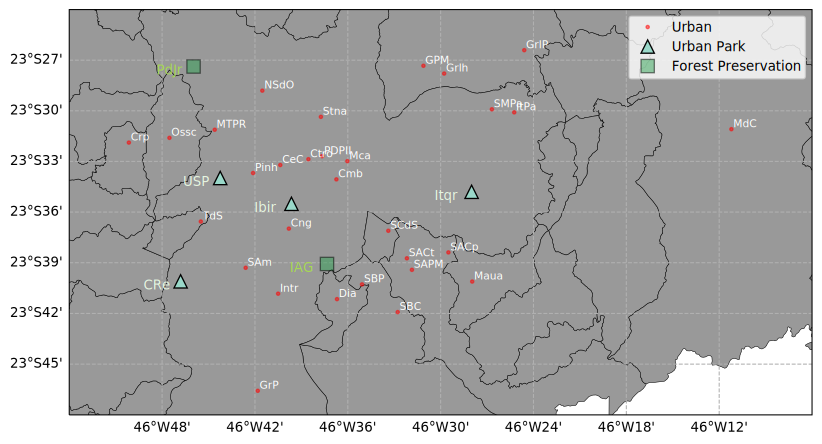
\includegraphics[width=1\textwidth]{fig/MASP_stations.pdf}
  		\caption{Air quality and meteorological stations network}

  		{\scriptsize Note:\\ The MASP map is in gray color. All stations except IAG belong to CETESB.}
  		\label{fig:mapStations}
	\end{figure}
	
  	\begin{figure}[htb]
		\includegraphics[width=1\textwidth]{fig/Stations_type_reduced.pdf}
  		\caption{Station classification type based on location in the S\~{a}o Paulo State. Maps Data: Google \copyright 2020, Maxar Technologies.}
  		\label{fig:station_types}
	\end{figure}
	
  \subsection{Air quality data}
  The period from 2014 to 2018 was analyzed, as shown in Figures~\ref{fig:Data} and \ref{fig:o3_years}.
  September and October presented higher hourly monthly mean surface ozone concentrations in many station types (e.g., Industry, Regional urban, Urban), as shown in Figure~\ref{fig:o3_time}.
  September presented more frequently higher surfer ozone concentrations than the other months and, for that reason, it can be considered the worst-case scenario.
  The maximum ozone concentration was reached at 15 hours (local time) in many station types (e.g., Forest preservation, Industry, Regional urban, and Urban).
  After 15 hours, during the evening, mean ozone concentrations decrease more than those recorded for December and January, as shown in Figure~\ref{fig:o3_time}.
  
  Regarding the interactions between surface ozone with other pollutants (CO, NO$_x$), Figure~\ref{fig:aqHour} shows charts by station type as hourly mean concentration based on data collected from September and October, 2018.
	The surface ozone reached its maximum levels between 14:00-15:00 hours (local time).
	CO and NO$_x$ (NO and NO$_2$) highest concentrations occurred at early morning (7:00-10:00 h) and evening (18:00-20:00 h) hours, positively correlated with the temporal distribution of emissions for light-duty and heavy-duty vehicles (Figure~\ref{fig:temp_distr}).
	Reduction of these pollutant concentrations between 11:00-19:00 hours is related to photochemical reactions that enhance ozone formation.
	Nocturnal ozone maximum concentration occurred around three and six hours (local time).
	This behavior was mentioned by \citet{Carvalho2015}, and can be associated with atmospheric transport from vertical levels, as it is mentioned in \citet{Mazzoli2013} and \citet{Andrade2017}.
	
	As mentioned in \citet{CETESB2019}, few stations monitor some hydrocarbons such as Benzene and Toluene (Figure~\ref{fig:HC_obs}).
	The hourly analysis shows a reduction of these VOC during the photochemical activity as shown in Figure~\ref{fig:hc_all_hour}.
  
  \begin{table}
	\centering
	\caption{CETESB stations considered to monthly analysis \\based on five years (2014-2018)}
	\label{tab:sta_year}
	\begin{tabular}{ll}
	\toprule
 	            Type &            Station \\
	\midrule
 Forest preservation &    Pico do Jaraguá \\
            Industry &           Paulínia \\
      Regional urban &  Campinas-Taquaral \\
      Regional urban &           Sorocaba \\
               Urban &         Interlagos \\
               Urban &        Carapicuíba \\
               Urban &  Parque D.Pedro II \\
               Urban &          Pinheiros \\
          Urban park &         Ibirapuera \\
          Urban park &           Itaquera \\
	\bottomrule
	\end{tabular}
   \end{table}
  
	
	\begin{figure}[!htb]
		\begin{center}
			\includegraphics[width=0.6\textwidth]{fig/aqHourSep_Urban.pdf}
			\includegraphics[width=0.6\textwidth]{fig/aqHourSep_Urban park.pdf}
			\includegraphics[width=0.6\textwidth]{fig/aqHourSep_Forest preservation.pdf}
		\end{center}
		\caption{Hourly mean concentrations for surface ozone (O$_3$), nitrogen monoxide (NO), nitrogen dioxide (NO$_2$), and carbon monoxide (CO) by station type in the MASP.}
		{\scriptsize Note. Shaded area corresponds to the standard deviation. }
		\label{fig:aqHour}
	\end{figure}
	
	\begin{figure}[hbt]
		\begin{center}
			\includegraphics{fig/byhour_all_polls.pdf}
		\end{center}
  		\caption{Hourly mean concentration by month (Sep-Oct, 2018), based on measurements in Pinheiros and S. André-Capuava stations.\\}
  		{\scriptsize Note: Toluene (Tol). Benzene (Ben). Shaded area corresponds to ozone concentration standard deviation.}
  		\label{fig:hc_all_hour}
	\end{figure}

  
  \subsection{Meteorological data}
  CETESB stations register hourly values for meteorological parameters such as surface temperature, relative humidity, wind speed and direction.
  However, these stations do not register hourly precipitation.
  Complementary, hourly data registered from the IAG climatological station in Água Funda was used for this study to compare with WRF-Chem model results.
  This data was requested on the IAG/USP station website: \\ \url{http://www.estacao.iag.usp.br/sol_dados.php}.\\
  The data was received as Excel files (hourly in rows and day in columns) and ordered as time series in rows and meteorological parameters in columns.
  Figure~\ref{fig:met_iag} in Appendix shows hourly time variation for September and October 2018 for eight meteorological parameters.
  Figure~\ref{fig:rain_cc_iag} in Appendix shows total daily rain and mean cloud cover; which in September (107 mm) was less than October (152 mm).
  According to \citet{Carvalho2015}, the weather condition in spring enhances ozone formation and is related to low cloud cover.
  September presented less values of cloud cover favoring the ozone formation due to photochemical activity.
  
  \section{Model performance evaluation}
  As recommended by \citet{Seinfeld2016}, three different performance index can be used to analyze the urban ozone models in the ability to reproduce the peak ozone concentrations, described below:
  
  \begin{itemize}
  	\item Analysis of predictions and observations paired in space and time.
  	\item Comparison of predicted and observed maximum concentrations.
  	\item Comparisons paired in space but not in time.
  \end{itemize}
  
Other recommendations are to use charts, plots, and statistical metrics for evaluating model results, letting us understand the model performance and its behavior, as suggested by \citet{Emery2017}.
  There are recommendations about statistics and benchmarks to assess photochemical model performance.
  \citet{Emery2017} analyzed statistical benchmarks applied to North American.
  For ozone, they recommended calculating statistics over temporal scales of one week (an episode), not longer than one month, and compared with recommended goals\footnote{"The more restrictive goals around the 33rd percentiles indicate statistical values that about one-third of top performing past applications in many U.S. modeling studies have met, and should be viewed as the best a model can be expected to achieve" \citep[defined in][]{Emery2017}.} and criteria\footnote{"The less restrictive criteria around the 67th percentile indicate statistical values that about two-thirds of past applications have met, and should viewed as establishing historical context that a majority of models have achieved" \citep[defined in][]{Emery2017}.} benchmarks shown in Table~\ref{tab:ozone_bench}.
  Although these statistical benchmarks were based on  North American modeling studies, \citet{Emery2017} recommendations are relevant to any such applications of state-of-science photochemical models.
  Therefore, they can be used for Brazil.
  In case one or two did not comply with the recommended criteria for Normalized Mean Bias (NMB), Normalized Mean Error (NME), or Pearson correlation coefficient (\textit{r}), the modeling application should not be considered "failure" \citep{Emery2017}.
  The same authors recommend to restrict periods when observations exceed a minimum threshold value ("cutoff"), particularly for ozone. As conclusion in the paper published by \citet{Emery2017}, they recommend:
  
  \begin{quote}
  	"applying a cutoff value of 40 ppb (observations) when calculating only NMB and NME for 1 hour ozone, for several physical and regulatory reasons beyond the need for statistical stability, but not for correlation as it is best characterized over the entire concentration distribution. The choice of 40 ppb is not absolute and should consider the chemical climatology of the region being modeled."
  \end{quote}
  
  On the other hand, even when the primary aim of this study is to understand ozone formation, it is also essential to consider meteorological conditions.
  Why do we need to evaluate meteorological results?  \citet{Emery2017} and \citet{Monk2019} suggest that it is essential due to its crucial role in the air quality simulations (e.g., ozone) since weather conditions are also a significant air quality driver.
  
  For this study, model results for September and October 2018 were compared with hourly measured data at each station.
  This evaluation let us to compare the analysis of modeled and observed values in space and time, suggested by \citet{Seinfeld2016}.
  Previously, units concentrations from model results (excluding CO) were converted from mixing ratio ppm(v) to $\mu$g~m$^{-3}$, using the following equation \citep{Seinfeld2016}:
  
  \begin{equation}
	Concentration ~[\mu g/m^3] = \frac{p ~M_i}{8.314~ T}\times \zeta _i ~[ppm] \label{eq:conv}
 \end{equation}
  
  Where $p$ is the atmospheric pressure in Pa (N~m$^{-2}$), M$_i$ is a molecular mass (g~mol$^{-1}$), $T$ is in Kelvin, and $\zeta _i$ is the mixing ratio in ppm, considering a molecular gas constant ($R$) equals to 8.1314 J K$^{-1}$~mol$^{-1}$ or Pa~m$^{-3}$~K$^{-1}$~mol$^{-1}$.
  Meteorological simulations of temperature and atmospheric pressure were used to convert concentration from ppm to $\mu$g~m$^{-3}$.
  
   The analysis of surface ozone was performed in two forms: 1-hr time series and the maximum daily 8-hr rolling mean (MDA8).
   Thus, the comparison of predicted and observed maximum concentrations is made based on MDA8 values for ozone concentrations through time plots by station types.
  Other pollutants as nitrogen oxides (NO, NO$_2$), CO, and toluene were also analyzed in time and space.
  We analyzed toluene only for some stations where it was measured during September and October 2018 period. 
  It is important to remark that the WRF-Chem model did not include benzene in the results.
  Therefore, it is excluded from the statistical analysis and the comparison with observations.
 
  Regarding meteorological evaluation, S\~{a}o Paulo state can be considered as a complex terrain due to areas with high altitudes (e.g., Pico do Jaragu\'{a}) and high buildings in the MASP.
  For this reason, meteorology model results were evaluated using specific statistical benchmarks suggested by \citet{Monk2019} for complex terrain (Table~\ref{tab:met_bench}).
  
  \begin{table}
	\centering
	\caption{Statistical benchmarks for surface ozone (1-hr or MDA8) \\ suggested by \citet{Emery2017}}
	\label{tab:ozone_bench}
	\begin{tabular}{lll}
  		\toprule
  		Statistical metric & Goal & Criteria \\
  		\midrule
  		NMB 	& <$\pm$5 \% 	& < $\pm$15 \% \\
  		NME    	& <15 \%		& < 25 \% \\
  		r		& > 0.75 \% 		& > 0.5 \% \\
  		\bottomrule
  		\multicolumn{3}{l}{\footnotesize Notes. Normalized Mean Bias (NMB), Normalized}\\
  		\multicolumn{3}{l}{\footnotesize Mean Error (NME), correlation coefficient (r).}
	\end{tabular}
 \end{table}
  
  \begin{table}
	\centering
	\caption{Statistical benchmarks for meteorology parameters suggested by \citet{Monk2019}}
	\label{tab:met_bench}
	\begin{tabular}{lll}
	\toprule
  	Parameter & Statistical metric & Complex terrain \\
 	 \midrule
  	Temperature [K]			& MAGE &  $\leq$ 3 \\
  		  					& MB   &  $\leq \pm$1\\
  	      					& IOA  &  $\geq$ 0.8 \\ 
  	Relative humidity   		& MAGE & < 20 \% \\
  							& MB   & < $\pm$10 \%\\
  							& IOA  &  $\geq$ 0.6\\
  	Wind speed [ms$^{-1}$]	& RMSE & $\leq$ 2.5\\
  							& MB   & $\leq \pm$1.5 \\
  							& IOA  & $\geq$ 0.6\\
  	Wind direction [degree] & MAGE & $\leq$ 55	\\
  							& MB   & $\leq \pm$10  \\
  	\bottomrule
  	\multicolumn{3}{l}{\footnotesize Notes. Mean Absolute Gross Error (MAGE), Mean Bian (MB), }\\
  	\multicolumn{3}{l}{\footnotesize index of agreement (IOA), Root Mean Square Error (RMSE).}
  	\end{tabular}
\end{table}

More details, such as utilities, can be found in Appendix~\ref{ap04}. Statistic equations are described as follows based on the description by \citet{Emery2017}:
  
  \begin{align}
  MAGE =&~ \frac{1}{N}\sum|P_j - O_j| \\
  MB = &~  \frac{1}{N}\sum(P_j - O_j)\\
  IOA = &~ 1 - \frac{\sum(P_j-O_j)^2}{\sum(|P_j+\overline{O}|+|O_j+\overline{O}|)^2}\\
  NMB =&~ \frac{\sum(P_j-O_j)}{\sum O_j}\times 100\\
  NME =&~ \frac{\sum|P_j-O_j|}{\sum O_j}\times 100\\
  r =&~ \frac{\sum[(P_j-\overline{P})\times(O_j-\overline{O})]}{\sqrt{\sum(P_j-\overline{P})^2\times \sum(O_j-\overline{O})^2}}
  \end{align} 
    
  \subsection{Hypothesis test for Pearson's r}
 The correlation coefficient (\textit{r}) gives us information about how two datasets have a linear relationship or not.
  A positive perfect correlation (+1) corresponds to all the pairs lying on a straight line with a positive slope when a scatter diagram is used.
  It is desired to achieve in air quality modeling (a perfect model!). 
  However, a few paired values could generate errors for the correlation coefficient, which could not be robust or significant.
  Significance and confidence interval can be calculated for correlation coefficient based on t-test (two-tailed).
  %, available in the Python function \verb|r_pearson_sign| as part of \verb|mod_stats.py| script.
   Based on \citet{Navidi2019} t-test statistical evaluation methodology, we defined Null (H$_o$) and Alternative hypothesis (H$_A$), considering an alpha ($\alpha$) equals to 0.05 for degree freedom (df) equals to n-2, where n is the number of paired values:
  \begin{itemize}
  	\item H$_o$: $\rho$ = 0 (samplings of x (obs) and y (mod) are not correlated)
  	\item H$_A$: $\rho$ $\neq$ 0
  \end{itemize}
  Where $\rho$ denotes the population correlation between x and y.
  Then, assuming that H$_o$ is true, a statistical test is computed and used to asses the strength of the evidence against H$_o$.
  Also, we compute the P-value of the test that is the probability and is also called the \textbf{observed significance level}.
  The P-value measures the plausibility of H$_o$.
  So, if the P-value is sufficiently small, we may be willing to abandon the assumption that H$_o$ is true and believe H$_A$ instead (rejecting the null hypothesis).
  As a practical rule, if the t critical value (calculated from $\alpha$=0.05 and n-2 degree freedom) is less than the t-statistic, we will reject the null hypothesis and accept the H$_A$.
  Therefore, we can state "there is enough evidence to conclude that there is a significant linear relationship between x (obs) and y (mod) because the correlation coefficient is significantly different from zero."
  The formula for the t-statistic value calculation is \citep{Navidi2019}:
  
  \begin{align}
  	t = \frac{r\sqrt{n-2}}{\sqrt{1-r^2}}
  \end{align}
  
  Where r is the sample correlation of the n points. 
  The t-statistic value has the same sign as the correlation coefficient.






  
  
  